\documentclass[tikz,border=2pt]{standalone}
\usepackage{amsmath}
\usepackage{pgfplots}
\pgfplotsset{compat=1.18}
\usetikzlibrary{arrows.meta}
\begin{document}
% Left: K = union of the half-lines through (1,0) and (0,1) is a cone, but the midpoint (1/2,1/2) of (1,0),(0,1) is not in K.
% Right: the halfspace x1+x2<=1 is convex but not a cone: (1,0) lies in it, 2(1,0)=(2,0) does not.
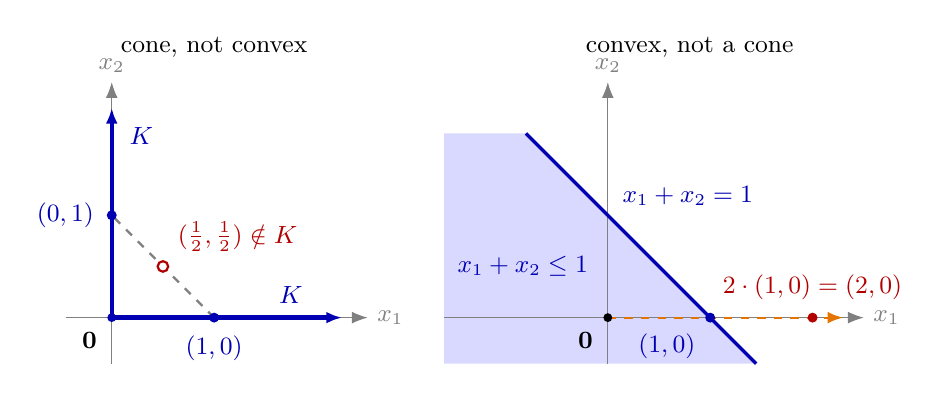
\begin{tikzpicture}[font=\small, >={Latex[length=2mm]}, x=1.3cm, y=1.3cm]
  % ---------- left panel: a cone that is not convex
  \begin{scope}
    \draw[gray, ->] (-0.45,0) -- (2.5,0) node[anchor=west] {$x_1$};
    \draw[gray, ->] (0,-0.45) -- (0,2.3) node[anchor=south] {$x_2$};
    \draw[blue!70!black, line width=1.6pt, ->] (0,0) -- (2.25,0);
    \draw[blue!70!black, line width=1.6pt, ->] (0,0) -- (0,2.05);
    \draw[gray, thick, dashed] (1,0) -- (0,1);
    \fill[blue!70!black] (1,0) circle (1.8pt);
    \fill[blue!70!black] (0,1) circle (1.8pt);
    \fill[blue!70!black] (0,0) circle (1.6pt);
    \node[blue!70!black, anchor=north] at (1,-0.08) {$(1,0)$};
    \node[blue!70!black, anchor=east] at (-0.08,1) {$(0,1)$};
    \node[anchor=north east] at (-0.05,-0.05) {$\boldsymbol{0}$};
    \node[blue!70!black, anchor=south west] at (0.08,1.6) {$K$};
    \node[blue!70!black, anchor=south] at (1.75,0.04) {$K$};
    \draw[red!70!black, thick, fill=white] (0.5,0.5) circle (1.9pt);
    \node[red!70!black, anchor=south west] at (0.55,0.55) {$(\tfrac{1}{2},\tfrac{1}{2})\notin K$};
    \node[anchor=south] at (1,2.45) {cone, not convex};
  \end{scope}
  % ---------- right panel: a convex set that is not a cone
  \begin{scope}[xshift=6.3cm]
    \fill[blue!15] (-1.6,-0.45) -- (1.45,-0.45) -- (-0.8,1.8) -- (-1.6,1.8) -- cycle;
    \draw[gray, ->] (-1.6,0) -- (2.5,0) node[anchor=west] {$x_1$};
    \draw[gray, ->] (0,-0.45) -- (0,2.3) node[anchor=south] {$x_2$};
    \draw[blue!70!black, very thick] (1.45,-0.45) -- (-0.8,1.8);
    \node[blue!70!black, anchor=south west] at (0.05,1.0) {$x_1+x_2=1$};
    \node[blue!70!black, anchor=east] at (-0.1,0.5) {$x_1+x_2\leq1$};
    \draw[orange!90!black, thick, dashed, ->] (0,0) -- (2.3,0);
    \fill (0,0) circle (1.6pt);
    \node[anchor=north east] at (-0.05,-0.05) {$\boldsymbol{0}$};
    \fill[blue!70!black] (1,0) circle (1.8pt);
    \node[blue!70!black, anchor=north east] at (0.95,-0.06) {$(1,0)$};
    \fill[red!70!black] (2,0) circle (1.8pt);
    \node[red!70!black, anchor=south] at (2,0.08) {$2\cdot(1,0)=(2,0)$};
    \node[anchor=south] at (0.8,2.45) {convex, not a cone};
  \end{scope}
\end{tikzpicture}
\end{document}
